Loci considered thus far have been smooth, regular curves.

\begin{proposition}
If $a/b>\alpha_4$ the locus of the Incenter of the 3-periodic's Orthic Triangle comprises four arcs of ellipses, connected at four corners.
\end{proposition}

To see this, let $T$ be a triangle, $T_h$ its Orthic\footnote{Its vertices are the feet of the altitudes.}, and $I_h$ be the latter's Incenter. It is well-known that if $T$ is acute $I_h$ coincides with $T$'s Orthocenter $X_4$. However, for obtuse $T$:

\begin{lemma}
$T_h$ has two vertices outside of $T$, and $I_h$ is ``pinned'' to the obtuse vertex
\label{lem:pinned}
\end{lemma}

This is a known result  \cite[Chapter 1]{coxeter67}, which we revisit in Appendix~\ref{app:orthic-incenter}. This curious phenomenon is illustrated in Figure~\ref{fig:orthic-incenter}. 

\begin{figure}
    \centering
    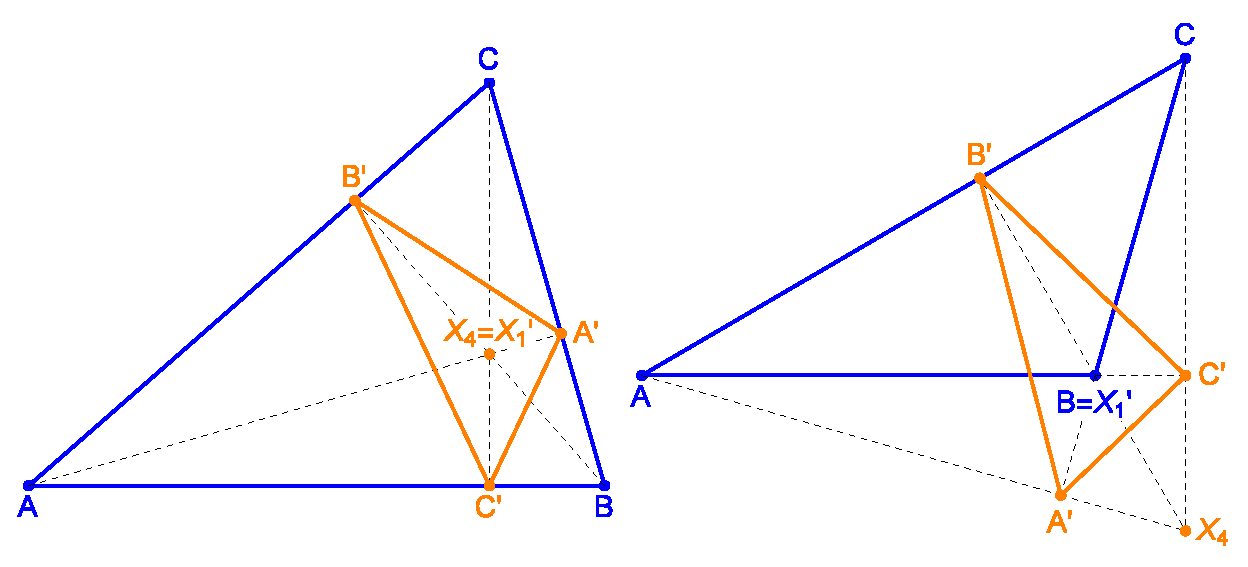
\includegraphics[width=.8\textwidth]{pics/1020_orthic_incenter.eps}
    \caption{\textbf{Left}: If $T=ABC$ is acute (blue), its Orthic $T'=A'B'C'$ is the so-called Fagnano Triangle \cite{rozikov2018-billiards}, whose properties include: (i) inscribed triangle of minimum perimeter, (ii) a 3-periodic of $T$, i.e., the altitudes of $T$ are bisectors of $T'$, i.e., the Orthic Incenter $X_1'$ coincides with the Orthocenter $X_4$. \textbf{Right}: If $T$ is obtuse, two of the Orthic's vertices lie outside $T$, and $X_4$ is exterior to $T$. $T'$ is the Orthic of {\em both} $T$ and {\em acute} triangle $T_e=A{X_4}C$. So the Orthic is the latter's Fagnano Triangle, i.e., $B$ is where both altitudes and bisectors meet. The result is that if $T$ is obtuse at $B$, the Incenter $X_1'$ of the Orthic is $B$. \textbf{Video}: \cite[PL\#06]{reznik2020-playlist-intriguing}}
    \label{fig:orthic-incenter}
\end{figure}

Assume $a/b>\alpha_4$. Since the 3-periodic family contains both acute and obtuse triangles, the locus of $I_h$ transition between acute and obtuse regimes:

\begin{center}
\small
\begin{tabular}{r|c|l}
 3-periodic & $X_4$ wrt EB & $I_h$ location \\ 
 \hline
 acute & interior & Orthocenter $X_4$ \\  
 right triangle & on it & right-angle vertex \\
obtuse & external (3-periodic Excenter) & obtuse vertex, on EB 
%\caption{Incenter behavior acute and obtuse 3-periodics.}
\end{tabular}

\end{center}

In turn, this yields a locus for $I_h$ consisting of four elliptic arcs connected by their endpoints in four corners, Figure~\ref{fig:orthic_incenter_locus}. Notice top and bottom (resp. left and right) arcs belong to the EB (resp. $X_4$ locus).

\begin{figure}
    \centering
    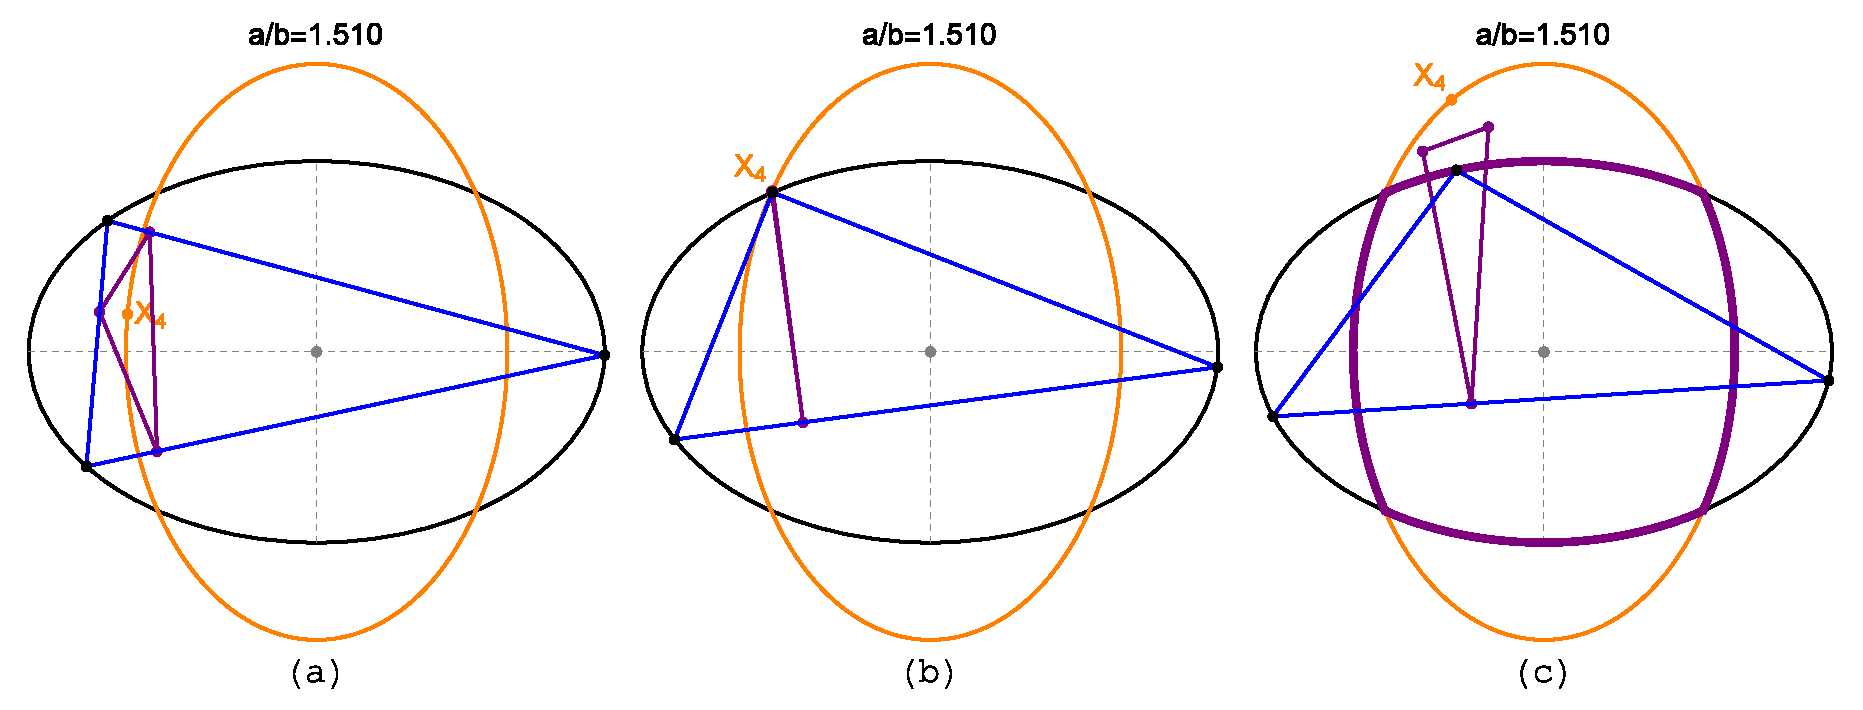
\includegraphics[width=\textwidth]{pics/1030_ort_loci_kink.eps}
    \caption{An $a/b>\alpha_4$ EB is shown (black). Let $T$ and $T_h$ be the 3-periodic and its Orthic Triangle (blue and purple, respectively). \textbf{(a)} $T$ is acute ($X_4$ is interior to the EB), and $I_h=X_4$. \textbf{(b)} $X_4$ is on the EB and $T$ is a right triangle. $T_h$ degenerates to a segment. \textbf{(c)} $X_4$ is exterior to the EB. Two of $T_h$'s vertices are outside $T$. $I_h$ is pinned to $T$'s obtuse vertex, on the EB. $X_4$ is an Excenter of the 3-periodic. The complete locus of $I_h$ comprises therefore 4 elliptic arcs (thick purple) duck-taped at the corners. \textbf{Video}: \cite[PL\#07]{reznik2020-playlist-intriguing}}
    \label{fig:orthic_incenter_locus}
\end{figure}

For the next proposition, 
let $\alpha_h^2$ (resp.~$1/\alpha_h'^2$) be the real root above 1 (resp.~less than 1) of the polynomial $1 + 12 x - 122 x^2 - 52 x^3 + 97 x^4$. Numerically, $\alpha_h{\simeq}1.174$ and $\alpha_h'{\simeq}2.605$.

%\textcolor{red}{ronaldo da pra trocar o $a_1$ %e $b_1$ (usados para os eixos do locus do %incentro) abaixo por talvez u,v ou outra %notacao?}

% TO INSERT: $a/b=\alpha_h''{\simeq}1.982$ the orthic is equilateral.

\begin{proposition}
At $a/b=\alpha_h$ (resp.~$a/b=\alpha_h'$), at the sideways (resp.~upright) 3-periodic, the Orthic is a right triangle, Figure~\ref{fig:right-orthic}. If $a/b>\alpha_h$ some Orthics are obtuse (a family always contains acutes).
\end{proposition}

\begin{proof}
The orthic of an isosceles triangle with vertices $A=(a,0),$ $B=(-u,v)$ and $C=(-u,-v)$ is the isosceles triangle with vertices:
\begin{align*}
A'=&(-u,0)\\
B'=&\left(\frac{-u(a+u)^2+v^2(2a+u) }{(a+u)^2+v^2},\frac{ v( (a+u)^2-v^2)}{(a+u)^2+v^2)}\right)\\
C'=&\left(\frac{-u(a+u)^2+v^2(2a+u) }{(a+u)^2+v^2},- \frac{v( (a+u)^2-v^2)}{(a+u)^2+v^2}\right)
\end{align*}
%
It is rectangle, if and only if, $\langle B'-A',C' -A'\rangle=0$. This condition is expressed by
$r(a,u,v)=(a+u)^2-v(2a+2u+v)=0.$

Using explicit expression to the 3-periodic vertices \cite{garcia2019-incenter}, obtain that  
$u= u(a,b)=a (\delta- {b}^{2})/({a}^{2}-{b}^{2})$ and $v=v(a,b)={b}^{2}\sqrt {2\delta-{a}^{2}-{b}^{2} 
}/({a}^{2}-{b}^{2}).
$
So it follows that $r(a,u,\simeq)=r(a,b)=97a^8-52a^6b^2-122a^4b^4+12a^2b^6+b^8=0.$
The same argument can be applied to the isosceles 3-periodic with vertices:
%
\begin{equation*}
    A=(0,b),\;\;B=(-v(b,a),-u(b,a)),\;\;C=(v(b,a),-u(b,a))
\end{equation*}
%
\noindent The associated orthic triangle will be rectangle, if and only if, $r(b,a)=0$.
\end{proof}


The obtuseness of 3-periodic Orthics is a complex phenomenon with several regimes depending on $a/b$, beyond the scope of this paper. It is explored in  \cite[PL\#08]{reznik2020-playlist-intriguing}.

%Figure~\ref{fig:orthic-orthic} provides experimental details. 

%\begin{figure}
%    \centering
%    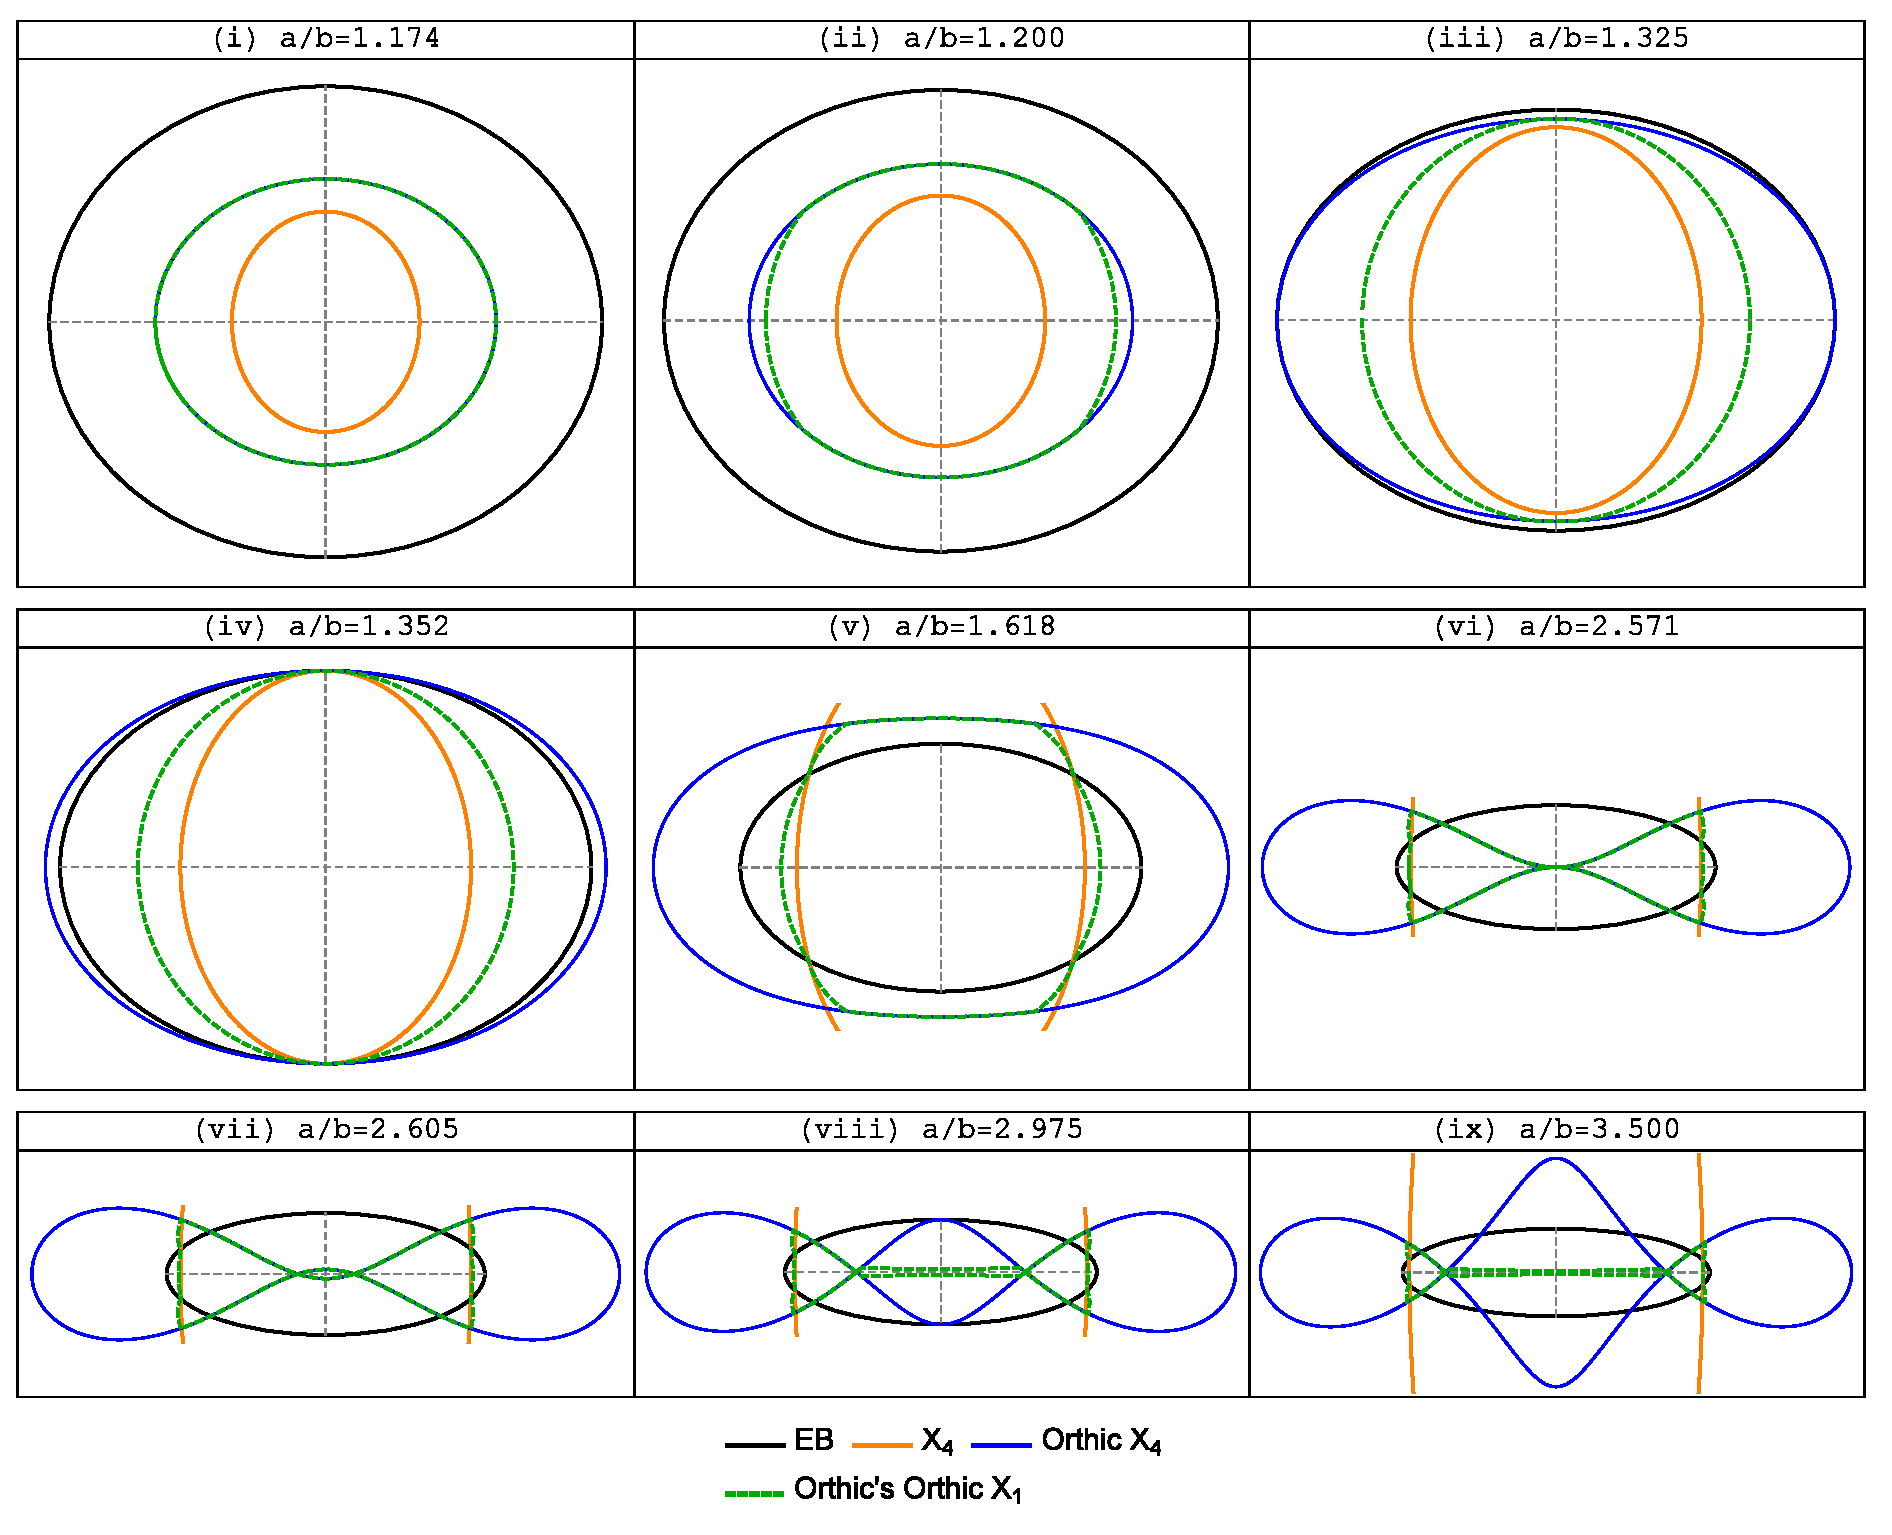
\includegraphics[width=.9\linewidth]{1085_pics_orthic_orthic.eps}
%    \caption{When are Orthics Obtuse? As before, this requires the Orthic Orthic's Incenter $X_1''$ (dashed green) to be detached from the Orthic's Orthocenter $X_4'$ (blue). Let $V$ (resp. $H$) denote either one of the two upright (resp. sideways) isosceles 3-periodics. Notable transitions occur at: (i) $a/b=\alpha_h{\simeq}1.174$, the locus of $X_1''$ is identical to that of $X_4'$, and at $H$, its Orthic is a right-triangle, Figure~\ref{fig:right-orthic} (left); (ii) $a/b>\alpha_h$, one can see $X_1''$ detaching from $X_4'$ indicating a region of obtuse Orthics about the $H$; (iii) At $a/b{\simeq}1.325$ the locus of $X_4'$ touches the EB's left and right vertices at the $H$; (iv) At $a/b=\alpha_4{\simeq}1.352$, the loci of $X_4$ of $X_4'$, and $X_1''$ touch the EB's top and bottom vertices, indicating $V$ are right-triangles and all Orthics not stemming from these are obtuse; (v) At $a/b>\alpha_4$, $X_1''$ tracks $X_4'$ about $V$, indicating some Orthics are acute; (vi) At $a/b{\simeq}2.571$, $X_4'$ two acute Orthics pass through the origin. Above this threshold, the locus of $X_4'$ becomes self-intersecting on the horizontal axis of the EB; (vii) At $a/b=\alpha_h'{\simeq}2.605$, $V$ yield right-triangle Orthics, Figure~\ref{fig:right-orthic} (right). Just above this threshold a new region of obtuse Orthics flares up about $V$; (viii) at $a/b{\simeq}2.965$ $X_4'$ of two obtuse Orthics touch top and bottom vertex of the EB at $V$; (ix) as $a/b$ increases, Orthics about $V$ become more and more obtuse (judging from the deviation between blue and dashed green curves), however two sideway regions of acute Orthic remain where $X_1''$ tracks $X_4'$: these are squeezed to the left and right of the self-intersections of $X_4'$ and the locus of $X_4$. \textbf{Video}: \cite[PL\#08]{reznik2020-playlist-intriguing}}
%    \label{fig:orthic-orthic}
%\end{figure}

\begin{figure}
    \centering
    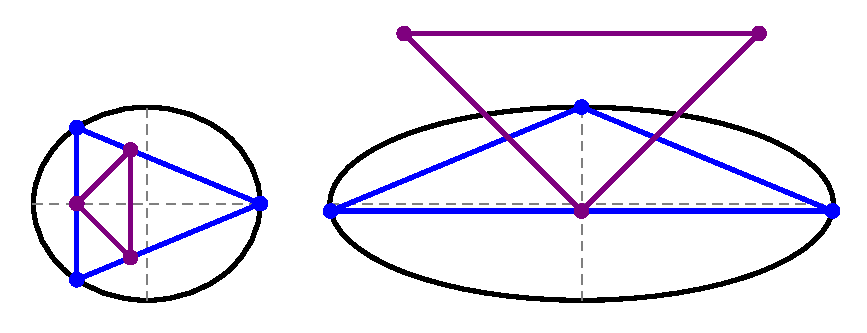
\includegraphics[width=.6\textwidth]{pics/1040_orthic_right_triangle}
    \caption{\textbf{Left}: At $a/b=\alpha_h{\simeq}1.174$, a sideways 3-periodic (blue) has a right-triangle Orthic (purple). If $a/b>\alpha_h$ some Orthics in the family are obtuse. \textbf{Right}: At $a/b=\alpha_h'{\simeq}2.605$, when the 3-periodic is an upright isosceles (obtuse since $a/b>\alpha_h$), its extraverted Orthic is also a right triangle.}
    \label{fig:right-orthic}
\end{figure}